\documentclass[polish,a4paper,twoside]{article}

\usepackage[utf8]{inputenc}
\usepackage[T1]{fontenc}
\usepackage{graphicx}
\usepackage[section]{placeins}

\author{Michał Kuźma\\[1cm]{\small Prowadzący: dr inż. Jerzy Stefanowski}}
\title{Hierarchical Classifier}                  

\begin{document}

% Front matter starts here
\pagestyle{empty}
\maketitle

\section{Wstęp}

Algorytmy uczenia maszynowego zdają się dzisiaj być wszechobecne. Od rozpoznawania twarzy podczas robienia zdjęć, przez automatyczne etykietowanie zdjęć, a skończywszy na alertach lekarskich ostrzegających o ryzyku wystąpienia choroby. Ta dziedzina nauki rozwija się na naszych oczach i jesteśmy skłonni powierzyć automatycznym klasyfikatorom coraz bardziej złożone i odpowiedzialne zadania. \\

Jednak pomimo dużego postępu i znacznego wzrostu precyzji klasyfikatorów na przestrzeni lat, niektóre przypadki wciąż są bardzo trudne do rozwiązania. Takim przypadkiem jest między innymi predykcja przy użyciu klasyfikatora nauczonego na zbiorze niezrównoważonym - takim, w którym znaczna większość przykładów przypisanych jest do jednej z dwóch klas. \\

Wspomniany problem niezrównoważonych zbiorów danych uczących znany jest od długiego czasu i zostało zaproponowanych wiele rozwiązań mających mu zaradzić. Od wykorzystania innych miar do oceny skuteczności algorytmu, przez różne metody wstępnego przetwarzenia danych, po klasyfikatory odporne na zjawisko zbiorów niezrównoważonych. \\

Trudniejszym zadaniem jest nauczenie klasyfikatora na zbiorze niezrównoważonym, w którym klasa mniejszościowa nie jest jednorodna (występuje w wielu skupiskach, a niekiedy jako pojedyncze przykłady otoczone większościowymi). Uważamy, że potencjalnym rozwiązaniem problemu może być zaproponowany przez nas klasyfikator hierarchiczny. \\

\section{Koncepcja projektu}

W publikacji z 2015 roku~\cite{minoritytypes-NapieralaStefanowski} zaproponowano następujacy podział przykładów klasy mniejszościowej:

\begin{itemize}
\item Przykłady bezpieczne (\emph{Safe}) -- Przykłady otoczone klasą mniejszościową, które bezpiecznie można uznać za mniejszościowe
\item Przykłady graniczne (\emph{Borderline}) -- Przykłady na granicy grupy klasy mniejszościowej, sąsiadują zarówno z przykładami klasy mniejszościowej, jak i większościowej
\item Przykłady rzadkie (\emph{Rare}) -- Przykłady klasy mniejszościowej stanowiące element małej grupy otoczonej większościowymi
\item Przykłady odosobnione (\emph{Outlying}) -- Pojedyncze obiekty klasy mniejszościowej otoczone w całości przez przykłady większościowe
\end{itemize}

\begin{figure}
\centering
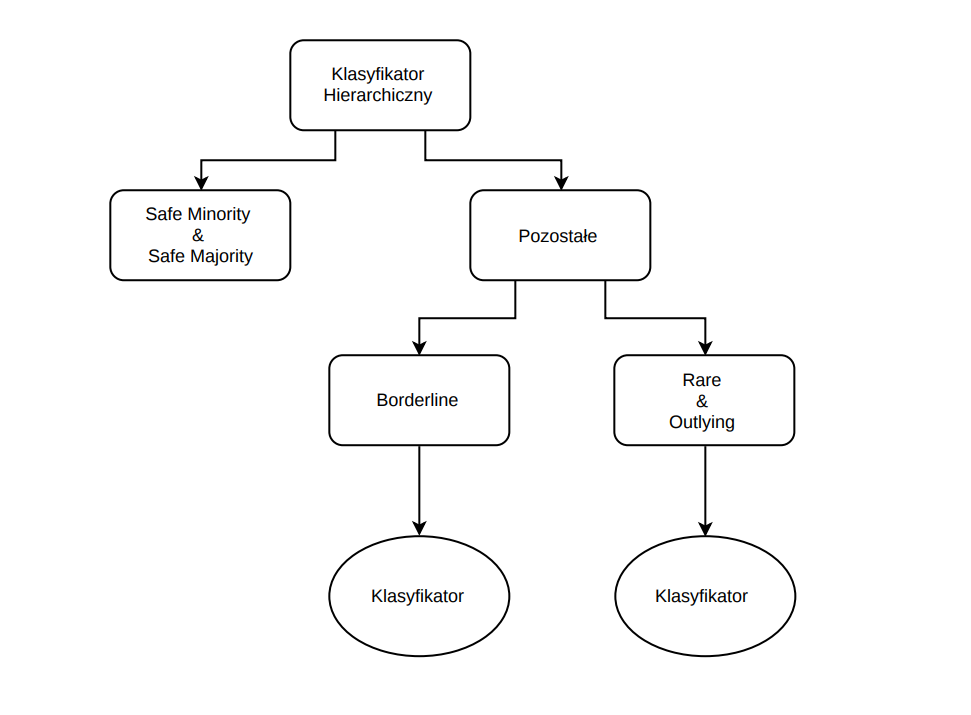
\includegraphics[width=\textwidth]{figures/hclassifier-diagram.png}
\caption{Schemat działania klasyfikatora hierarchicznego}
\label{fig:hclassifier-diagram}
\end{figure}

Zaproponowany przez nas klasyfikator uczy się i dokonuje predykcji w sposób hierarchiczny, jak przedstawia figura \ref{fig:hclassifier-diagram}. Na pierwszej warstwie zbiór dzielony jest na przykłady bezpieczne (tak z klasy mniejszościowej, jak i z większościowej), które mogą być wprost zaetykietowane i pozostałe. Te są dalej dzielone na graniczne i "niebezpieczne" (\emph{Rare} i \emph{Outlying}). Oba zbiory stanowią zestawy uczące dla prostych klasyfikatorów. \\

Zgodnie z sugestią z \cite{minoritytypes-NapieralaStefanowski} przykłady etykietowane są określonym typem w procesie analizy sąsiedztwa $k$ najbliższych sąsiadów. \\

\section{Wyniki eksperymentów}

Celem eksperymentów było porównanie wyników czystego drzewa decyzyjnego C4.5 i opartego na nim klasyfikatora hierarchicznego. Główny nacisk położyliśmy na czułość dla klasy mniejszościowej (stosunek poprawnie sklasyfikowanych przykładów mniejszościowych do wszystkich obiektów tej klasy). \\

Eksperymenty przeprowadzono na zbiorach rzeczywistych, które charakteryzują się występowaniem niejednorodnej klasy mniejszościowej. Wykorzystane zbiory danych:

\begin{itemize}
\item \emph{Seismic bumps}
\item \emph{Haberman}
\item \emph{Solar flare}
\item \emph{CMC}
\end{itemize}

\subsection{Zbiór \emph{seismic bumps}}

\begin{table}[!htb]
\centering
{\small
\begin{tabular}{|r|c|c|}
\hline
\textbf{Oryginalna \textbackslash Predykcja} & \textbf{Mniejszościowa} & \textbf{Większościowa} \\ \hline
\textbf{Mniejszościowa} & 11 & 159 \\ \hline
\textbf{Większościowa} & 39 & 2375 \\ \hline
\multicolumn{3}{}{} \\ \hline
\textbf{Ważona czułość} & \multicolumn{2}{c|}{0.923375} \\ \hline
\textbf{Czułość mniejszościowej} & \multicolumn{2}{c|}{0.064706} \\ \hline
\textbf{Czułość większościowej} & \multicolumn{2}{c|}{0.983844} \\ \hline
\end{tabular}
}
\caption{Macież pomyłek i czułości klasyfikatora hierarchicznego}
\label{tab:seismic_bumps:h}
\end{table}

\begin{table}[!htb]
\centering
{\small
\begin{tabular}{|r|c|c|}
\hline
\textbf{Oryginalna \textbackslash Predykcja} & \textbf{Mniejszościowa} & \textbf{Większościowa} \\ \hline
\textbf{Mniejszościowa} & 0 & 170 \\ \hline
\textbf{Większościowa} & 2 & 2412 \\ \hline
\multicolumn{3}{}{} \\ \hline
\textbf{Ważona czułość} & \multicolumn{2}{c|}{0.933437} \\ \hline
\textbf{Czułość mniejszościowej} & \multicolumn{2}{c|}{0.000000} \\ \hline
\textbf{Czułość większościowej} & \multicolumn{2}{c|}{0.999171} \\ \hline
\end{tabular}
}
\caption{Macież pomyłek i czułości drzewa decyzyjnego}
\label{tab:seismic_bumps:c}
\end{table}

\subsection{Zbiór \emph{haberman}}

\begin{table}[!htb]
\centering
{\small
\begin{tabular}{|r|c|c|}
\hline
\textbf{Oryginalna \textbackslash Predykcja} & \textbf{Mniejszościowa} & \textbf{Większościowa} \\ \hline
\textbf{Mniejszościowa} & 19 & 62 \\ \hline
\textbf{Większościowa} & 15 & 210 \\ \hline
\multicolumn{3}{}{} \\ \hline
\textbf{Ważona czułość} & \multicolumn{2}{c|}{0.748366} \\ \hline
\textbf{Czułość mniejszościowej} & \multicolumn{2}{c|}{0.234568} \\ \hline
\textbf{Czułość większościowej} & \multicolumn{2}{c|}{0.933333} \\ \hline
\end{tabular}
}
\caption{Macież pomyłek i czułości klasyfikatora hierarchicznego}
\label{tab:haberman:h}
\end{table}

\begin{table}[!htb]
\centering
{\small
\begin{tabular}{|r|c|c|}
\hline
\textbf{Oryginalna \textbackslash Predykcja} & \textbf{Mniejszościowa} & \textbf{Większościowa} \\ \hline
\textbf{Mniejszościowa} & 24 & 57 \\ \hline
\textbf{Większościowa} & 29 & 196 \\ \hline
\multicolumn{3}{}{} \\ \hline
\textbf{Ważona czułość} & \multicolumn{2}{c|}{0.718954} \\ \hline
\textbf{Czułość mniejszościowej} & \multicolumn{2}{c|}{0.296296} \\ \hline
\textbf{Czułość większościowej} & \multicolumn{2}{c|}{0.871111} \\ \hline
\end{tabular}
}
\caption{Macież pomyłek i czułości drzewa decyzyjnego}
\label{tab:haberman:c}
\end{table}

\subsection{Zbiór \emph{solar flare}}

\begin{table}[!htb]
\centering
{\small
\begin{tabular}{|r|c|c|}
\hline
\textbf{Oryginalna \textbackslash Predykcja} & \textbf{Mniejszościowa} & \textbf{Większościowa} \\ \hline
\textbf{Mniejszościowa} & 2 & 41 \\ \hline
\textbf{Większościowa} & 3 & 1020 \\ \hline
\multicolumn{3}{}{} \\ \hline
\textbf{Ważona czułość} & \multicolumn{2}{c|}{0.958724} \\ \hline
\textbf{Czułość mniejszościowej} & \multicolumn{2}{c|}{0.046512} \\ \hline
\textbf{Czułość większościowej} & \multicolumn{2}{c|}{0.997067} \\ \hline
\end{tabular}
}
\caption{Macież pomyłek i czułości klasyfikatora hierarchicznego}
\label{tab:solar_flare:h}
\end{table}

\begin{table}[!htb]
\centering
{\small
\begin{tabular}{|r|c|c|}
\hline
\textbf{Oryginalna \textbackslash Predykcja} & \textbf{Mniejszościowa} & \textbf{Większościowa} \\ \hline
\textbf{Mniejszościowa} & 0 & 43 \\ \hline
\textbf{Większościowa} & 0 & 1023 \\ \hline
\multicolumn{3}{}{} \\ \hline
\textbf{Ważona czułość} & \multicolumn{2}{c|}{0.959662} \\ \hline
\textbf{Czułość mniejszościowej} & \multicolumn{2}{c|}{0.000000} \\ \hline
\textbf{Czułość większościowej} & \multicolumn{2}{c|}{1.000000} \\ \hline
\end{tabular}
}
\caption{Macież pomyłek i czułości drzewa decyzyjnego}
\label{tab:solar_flare:c}
\end{table}

\subsection{Zbiór \emph{cmc}}

\begin{table}[!htb]
\centering
{\small
\begin{tabular}{|r|c|c|}
\hline
\textbf{Oryginalna \textbackslash Predykcja} & \textbf{Mniejszościowa} & \textbf{Większościowa} \\ \hline
\textbf{Mniejszościowa} & 85 & 248 \\ \hline
\textbf{Większościowa} & 99 & 1041 \\ \hline
\multicolumn{3}{}{} \\ \hline
\textbf{Ważona czułość} & \multicolumn{2}{c|}{0.764426} \\ \hline
\textbf{Czułość mniejszościowej} & \multicolumn{2}{c|}{0.255255} \\ \hline
\textbf{Czułość większościowej} & \multicolumn{2}{c|}{0.913158} \\ \hline
\end{tabular}
}
\caption{Macież pomyłek i czułości klasyfikatora hierarchicznego}
\label{tab:cmc:h}
\end{table}

\begin{table}[!htb]
\centering
{\small
\begin{tabular}{|r|c|c|}
\hline
\textbf{Oryginalna \textbackslash Predykcja} & \textbf{Mniejszościowa} & \textbf{Większościowa} \\ \hline
\textbf{Mniejszościowa} & 104 & 229 \\ \hline
\textbf{Większościowa} & 87 & 1053 \\ \hline
\multicolumn{3}{}{} \\ \hline
\textbf{Ważona czułość} & \multicolumn{2}{c|}{0.785472} \\ \hline
\textbf{Czułość mniejszościowej} & \multicolumn{2}{c|}{0.312312} \\ \hline
\textbf{Czułość większościowej} & \multicolumn{2}{c|}{0.923684} \\ \hline
\end{tabular}
}
\caption{Macież pomyłek i czułości drzewa decyzyjnego}
\label{tab:cmc:c}
\end{table}

\FloatBarrier
\section{Wnioski}

Na chwilę obecną klasyfikator w zależności od zbioru osiąga większą lub mniejszą dokładność od drzewa decyzyjnego. Dalsze prace są wskazane. \\

\bibliographystyle{plain}
\bibliography{bibliography}

\end{document}